\chapter{Light confinement in sub-wavelength nano-structure} \label{LM}


\section{Light and Nanowire} \label{corrections}


\subsection{Leaky Mode Resonance}
\label{sec:hydrogen}

Interaction of light with a dielectric or metallic cylindrical medium is
analyzed by solving Maxwell's equations with the appropriate boundary
conditions in the classical waveguide theory [80] which leads to highly
confined modes in optical fibers and microscale dielectric resonators. In an
infinitely long cylinder, even at deep sub-wavelength diameters this results in
a “characteristic equation” the solution to which are the transverse magnetic
(TM) and transverse electric (TE) resonant modes. We can define the
electromagnetic modes of localized resonators as time-harmonic solutions of the
form  to the source-free Maxwell equations. This solution shows that the
longitudinal field component distributes outside the NW, and is in resonance
with the natural modes, such as TE11, TM02, etc., supported by the NW. These
modes have been termed leaky-mode resonances (LMR) [81, 82], and provide an
intuitive tool to facilitate the understanding and optimization of the
resonance effect in such nano-structures.  We replicate these results using
MEEP, a widely used open-source finite-difference time-domain (FDTD) simulation
package [83], to identify how light is confined in an infinitely long GaAs
nanowire. The top row of Fig. 1 shows several configurations of TM LMR modes
for a NW with diameter of 220nm, with excitation single wavelength light being
incident parallel to the NW axis. The blue and red color codes represent the
polarization of the electric fields. The TE modes are primarily identical to
the TM modes shown here with the electric and magnetic fields exchanged. If the
light is incident with an arbitrary angle, then so-called hybrid HE and EH
leaky modes will be excited instead of the pure TE or TM mode.  The bottom row
of Fig. 1 shows the directional energy flux density of the electromagnetic
field, the Poynting vector, at different time frames with light being incident
perpendicular to the NW axis from the right side. The light is seen to
propagate from the right and then mostly remain confined at the left part of
the cylinder. It is notable that in either case the light energy is spatially
distributed along the cross section of the wire but, as expected from a 2D
treatment does not vary axially. Figure 1 demonstrates that the LMR can gently
confine light within subwavelength semiconductor nano-structures, similar to
the intuitive ray-optics picture of multiple total internal reflections from
the periphery of the cylinder. As shown by in Ref. [81], these LMRs depend on
the radius and the height of the dielectric, which allows ‘light engineering’
of the nanowires so as to increase its absorption efficiency at pre-determined
wavelength, e.g., to maximize absorption of sunlight spectrum for  higher
efficiency solar cells, or to radiate as optical antennas. 

\subsection{Whispering Gallery Modes}
\label{sec:host}

Infinitely long cylindrical or hexagonal NW structures can also support
Whispering Gallery (WG) modes [78, 79, 84-90]. To calculate the resonant WGMs,
Maxwell’s equations have to be solved numerically [91] taking into
consideration the spectral dependence of the material of interest’s index of
refraction. However, we can deduce a simple plane-wave model from theoretical
derivations, and the relationship between resonance wavelength λ and the
corresponding mode serial number N can be obtained [92]. The WG modes can also
reflect and confine light in the (subwavelength) nanostructure by total
internal reflection from the curvature of the structure boundaries. However, a
light wave can interfere with itself only when having completed one full
circulation within the resonator, which means only the light with one or
multiple wavelengths are allowed to perform multiple circulations generating a
standing wave. Figure 2 from reference 85 shows near-field intensity patterns
of low-order TM polarized hexagonal WGMs for n=1 and refractive index =2.1.
Each mode pattern is labeled by its respective mode number m (lower right
number) and its symmetry class (upper right symbol).  For comparison, four mode
patterns of the circular cavity are given in the upper left and lower right
together with their angular mode number. We again observe the radial spatial
dependence of light intensity. Furthermore, the low order WG modes of hexagonal
NWs are essentially similar to the cylindrical ones, but for higher order modes
additional features will arise on the facets of the hexagonal NWs [85].
Simulation results also show little difference between WG mode and Leaky modes
in lower order modes for both hexagonal and cylindrical structures. As with the
LMR, the resonant WG modes have been used as the basis for a precise
theoretical explanation of the enhanced optical behavior of hexagonal NWs, such
as enhanced light absorption [81, 93-96] and emission [78, 97-99]. Furthermore,
these numerical solutions have lead to reproduction of experimental resonance
spectra, e.g., polarization-resolved micro-photoluminescence (µ-PL) and
cathodeluminescence (CL) spectroscopy.  \subsection{Fabry-Perot Resonant Mode}
The above analysis and results apply to long structures, hence, provide
two-dimensional radial modes, independent of the NW axis. However, light
confinement has strong axial dependence, necessitating three-dimensional
analysis of the cavity modes. FDTD simulation in 3D are used to identify the
axial dependence of resonant modes in these nano-structures, revealing modes
which are volumetric in nature.  Fabry-Perot (FP) modes have been analyzed for
sub-microcavity, or nano-cavity, NWs with cylindrical or hexagonal structures,
specifically in order to determine the axial dependence of the resonance modes
[100]. At least two mirrors are needed to construct the reflection structure
inside the cavity, whether they are the top and bottom ends, i.e., the air and
substrate interfaces with the nanowire, or any of the two opposite facets along
the nanowire axis. For subwavelength structures, the longitudinal WG modes have
high scattering losses due to diffraction, and axial FP waveguide modes will
dominate [90]. However, due to small difference of the refractive index between
the substrate and the nanowire dielectric, the existence of the FP mode will
only be valid if the nanowire has relatively large radii, e.g., larger than 200
nm [101]. Under these conditions, besides the top and bottom ends, the lateral
facets of nanowire can also be treated as two parallel slabs, and with the
dielectric in between, it can support the FP mode with mode spacing inversely
related to the nanowire length. An application of this analysis is in the
design of NW lasers, since the optical cavity modes are observed at threshold
for lasing, and have been investigated for both optical and electrical pumped
cases [102, 103]. As a results the FP resonance mode based nanoscale lasers are
not only capable of covering a wide spectral regions, but can also can be
integrated as single or multi-color laser source arrays in silicon based
photonic integrated circuit or microelectronic devices [102,103]. However, the
FP modes supported by the nano-cavity structure have relatively small quality
factor due to the small difference of the refractive indices of the substrate
and the NWs. In order to address this issue,  Bragg gratings can be produced at
the NW ends, alternatively, NWs can be placed on metal substrates in order to
increase the FP resonance peak intensity by more than one order of magnitude
compared to those on Si substrates [104].  \subsection{Helical Resonance Modes}
Nano needles of III-V material grown on heterogeneous substrates are
optoelectronic devices which have shown interesting optical behavior, including
lasing, at room temperature [105]. Figure 3 (A) shows SEM image of a nano-laser
grown on silicon substrate that has subwavelength dimensions on all sides.
Analysis of light propagation introduced by shows that unlike the traditional
WG mode that lack vertical structure, there is net propagation in axial
direction in these structures which leads to  volumetric resonant modes which
are termed helical mode resonances [105]. The schematic Fig. 3(B) suggests a
helical ray path with nearly total internal reflection at the
nanopillar-silicon interface due to the glancing angle of incidence from the
hexagonal facets of the nano-laser shown in Fig. 3(A). As such, the faceted
shape of the structure affects the optical cavity properties. FDTD-simulated
field profile shows a hexagonal WG-like mode pattern  in the transverseplane as
in Fig. 3 (C), which arises from strong azimuthal components of helical modes.
Figure 3 (D) shows first-order  and higher-order standing waves’ axial
variation. The radial mode number (first number, m) describes the transverse
field pattern for WG modes, and the axial mode number (second number, n)
describes the axial standing wave as is the case for Fabry-Perot resonances. It
is seen that light or optical field can be well confined in the nanostructure
even with low index contrast at the dielectric interface thus producing the
nano-resonators needed for lasing. Although the quality (Q) factors of such
nanostructure are usually not large, these helically propagating cavity modes,
provide an optical feedback mechanism without the sophisticated mirror
structures of the vertical cavity surface emitting lasers (VCSEL’s).
Additionally, since the nanowires are heteroepitaxially grown on different
substrates, they enable heterogeneous integration of photonic emitters and
silicon based computational circuitry.  Whereas traditional FP modes are
inhibited by the interface between semiconductor nanostructure and the silicon
substrate, such unique optical structures have been proposed as an avenue for
engineering and integrating on-chip nanophotonic devices. 

\section{Volumetric Modes} \label{sed} The diameter of the nanostructures which
can support the helical resonance modes is near the Rayleigh limit, around the
boundary of the validity of ray-optics. FDTD analysis can be applied to deeper
subwavelength structure in order to identify the cavity modes which are by
nature volumetric, i.e., axially dependent.  Figure 4 shows simulation results
for various diameters of hexagonal structure of 1 m length.  Incident
radiation with 532 nm wavelength is nearly parallel to the wire axis and
different modes are displayed for different radii. Top row shows radial spatial
dependence at the middle of the wire axis, and the bottom row shows the axial
dependence. Top row results are similar to Figures 1-2, and the bottom row
shows that the light can be confined in volumetric resonance mode in both
transverse plane and longitudinal plane even with sub-wavelength diameter of
these hexagonal NWs. Unlike helical modes, the explanation of resonance  need
not rely on an intuitive ray-optics description based on the grazing angle of
incident light, but shows similar results in how the deep subwavelength
structures can confine the light and produce a resonant cavity without having
sophisticated mirrors at the end facets. In this respect nano-cavities of
as-grown nanowires outperform microcavities of VCSELs.  \subsection{Nanocavity
Geometry Dipendence}

\subsection{Light Engineering of Nanocavities}

Dependence of the resonant modes on the cavity geometry offers an important
degree of freedom to engineer a cavity for particular optical properties.
Figure 6 shows the dependence of three volumetric TM resonant modes’ excitation
wavelengths with radius. In this spectral range, only lower TM modes can be
excited with smaller radii, e.g., r = 40 nm and 60 nm, however, as the radius
increases, higher order modes can be excited, and the optical power
corresponding to the lower order modes will be reduced. We observe redshift of
these volumetric TM modes with increasing NW radius. Also, the wavelength
variation of TM1n mode is much larger compared to TM2n and TM3n modes. These
observations demonstrate the feasibility to engineer the volumetric mode at
certain wavelength, i.e., allow us to optimize absorption or emission at a
desired frequency or certain incident optical power  by controlling the radius
and/or length of a NW thus providing the ability to engineer the absorption
spectrum in order to match desired properties.

iThe dependence of the resonant modes on NW radius also suggests the
interesting possibility of having tapered structures which can support more
than one resonant mode, thus be able to optimize the spectrum of interest.  The
metalorganic vapor phase epitaxy (MOVPE) or vapor liquid solid (VLS) growth
methods are readily capable of forming nanowires with tapered sidewalls. The
resultant cavity, however, does not support the superposition of the modes
present in cylindrical structures of the same diameter; in fact tapered
sidewalls have been identified as the primary loss mechanism for these
sub-wavelength cavities.  The effect of  tapering has been studied for
nanopillars that were grown on a silicon substrate with average 5° angles
between opposite sidewalls; vertical field profiles for ,  and  modes are shown
in Fig. 7 [105]. The modes are primarily confined at the base, and become less
resonant as they propagate upwards with decreasing of the radius at top.
Higher-order axial modes generally have lower quality factor. Physically, the
stronger Fabry-Perot characteristic of higher-order axial modes means that
their effective longitudinal wave-vector components become stronger, causing
larger penetration and loss into the substrate. Nevertheless, from a different
perspective, multi-mode resonances can be achieved within certain wavelength
range by controlling the tapering angle in order to form small varying radius
along the nanostructure axial direction. One can also red- or blue-shift the
resonance peaks, since these volumetric resonance modes are dependent on
transverse dimensions. Thus, intentioned tapering offers an alternative way to
engineering the multi-mode resonances and finer tunability of these resonance
peaks.

\begin{figure}
  \caption{Cylindrical Nanowire Ez with different Mode number}
  \centering
  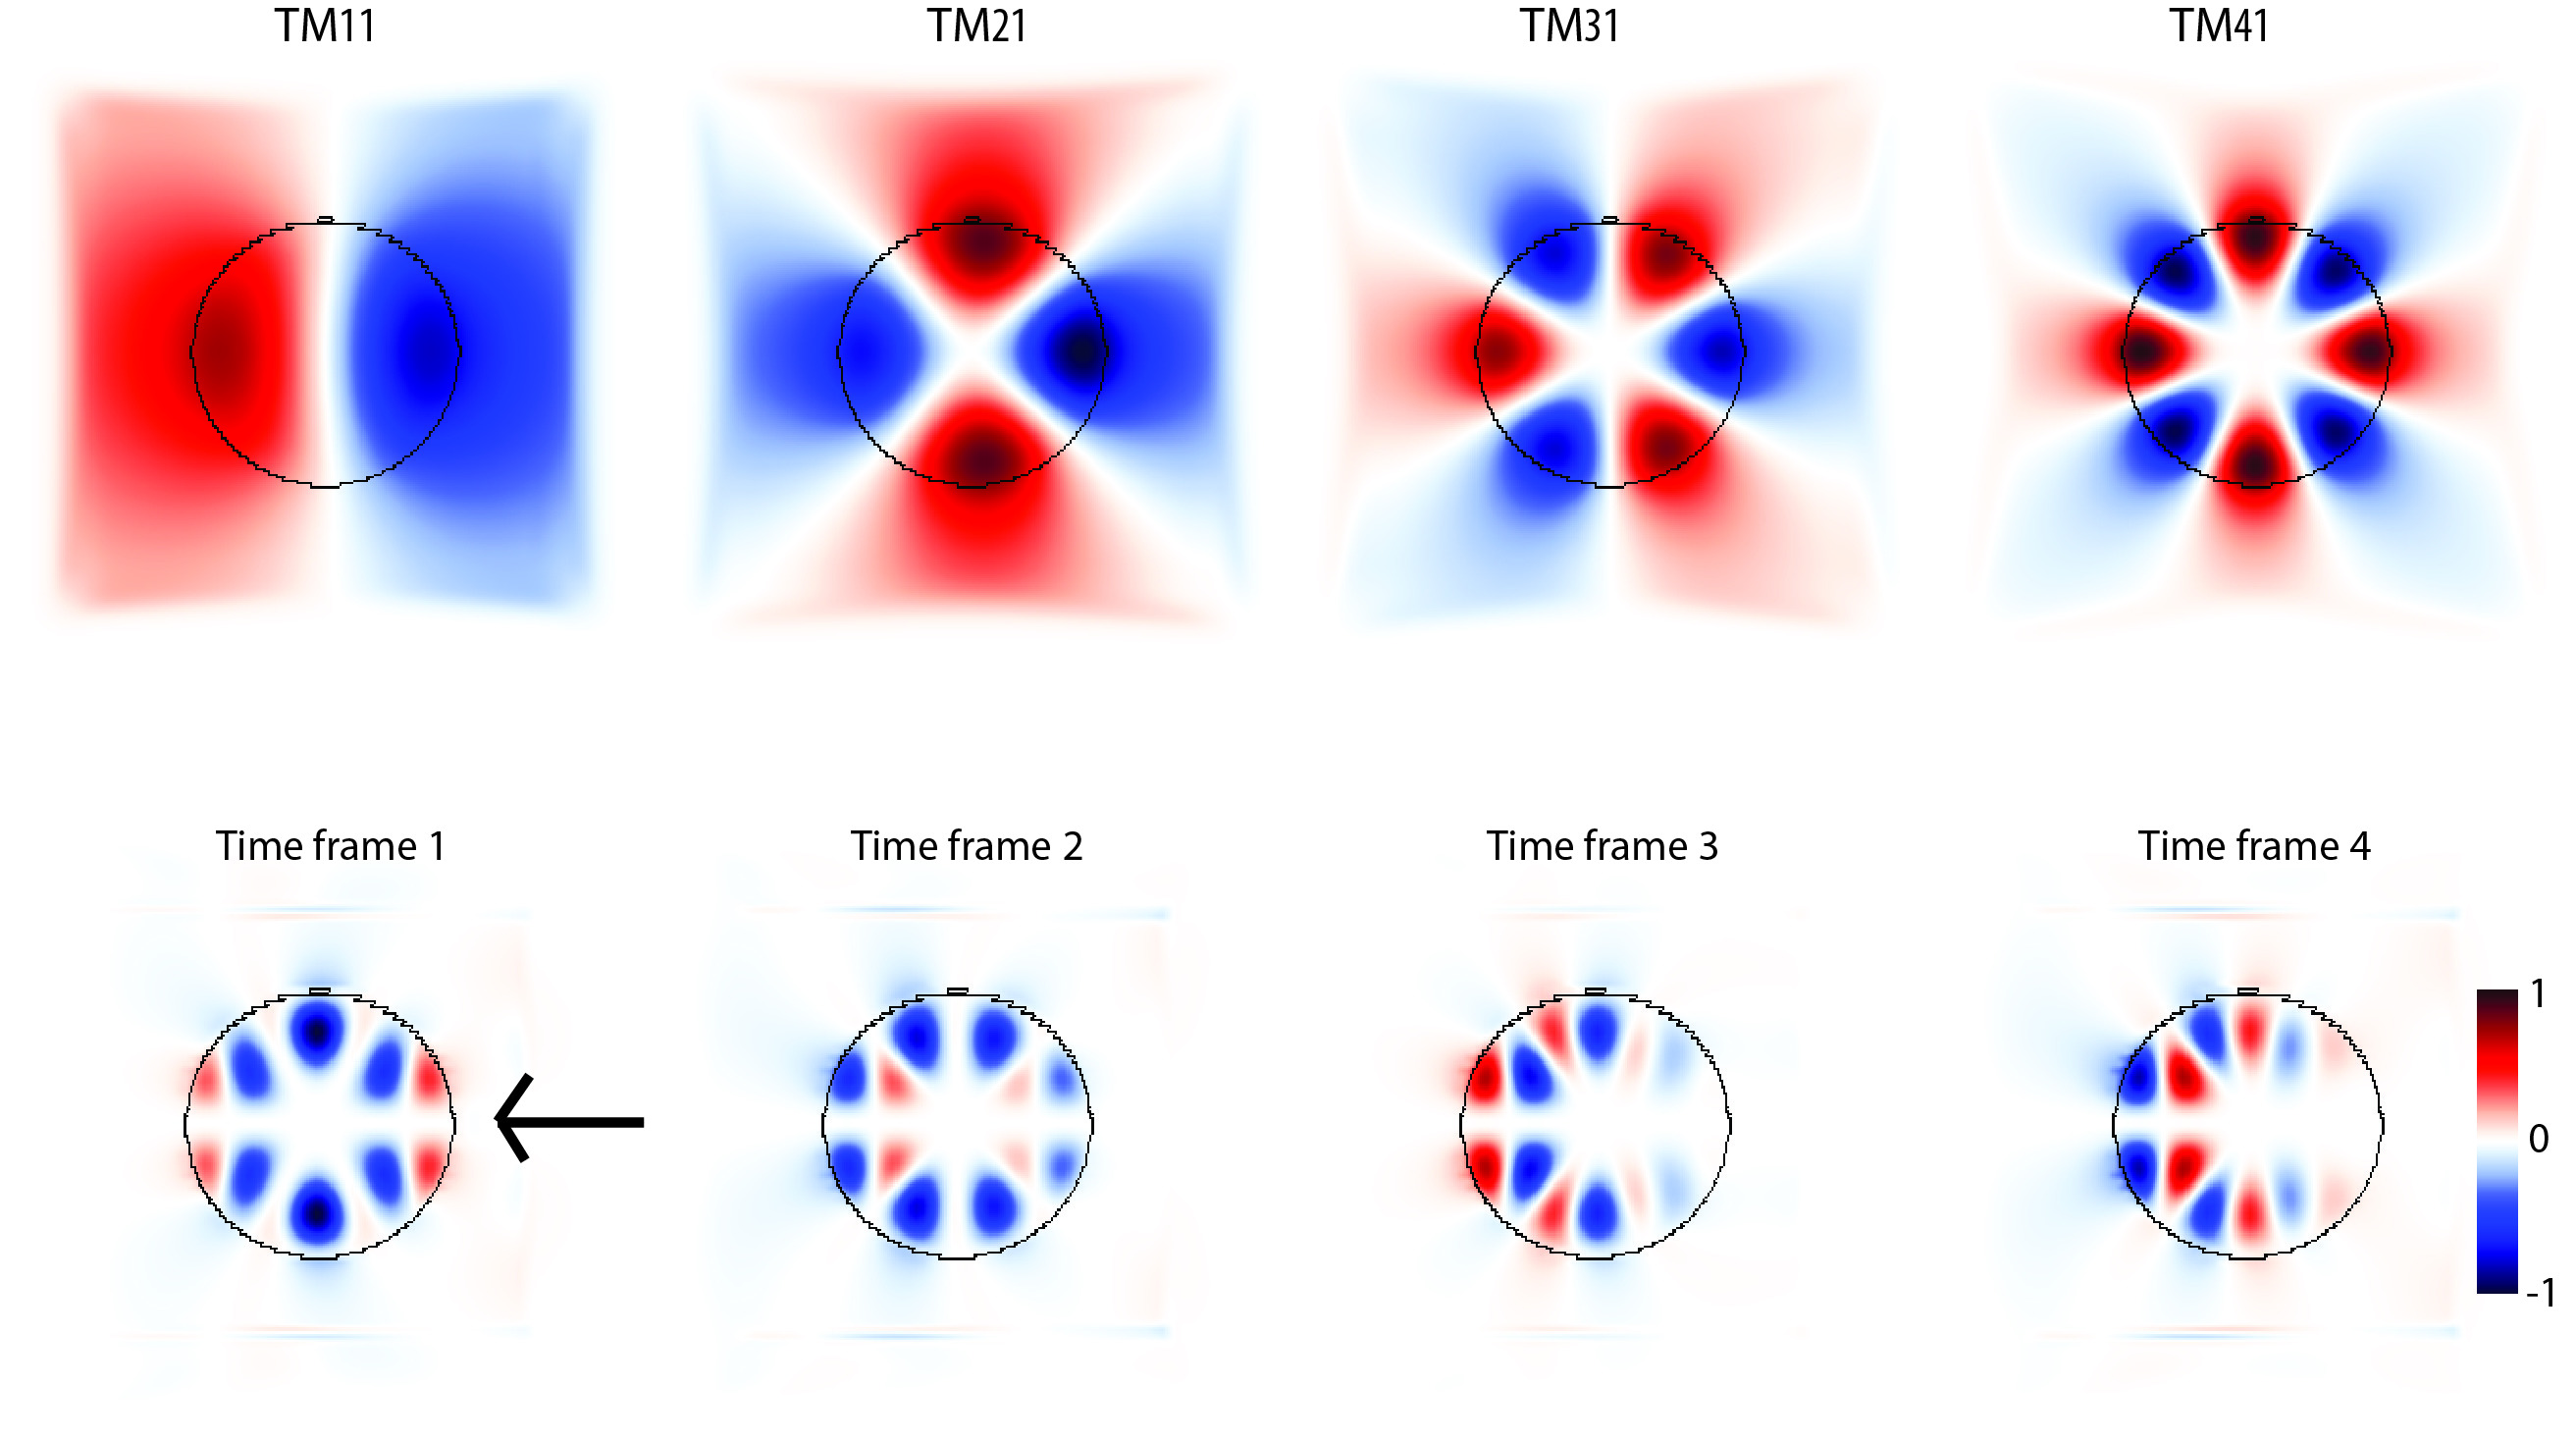
\includegraphics[width=\textwidth]{pictures/LM/CylindEz}
  \label{CylindEz}
\end{figure}

\begin{figure}
  \caption{Simulation Schematic for Cylindrical and Hexagonal Nanowires}
  \centering
  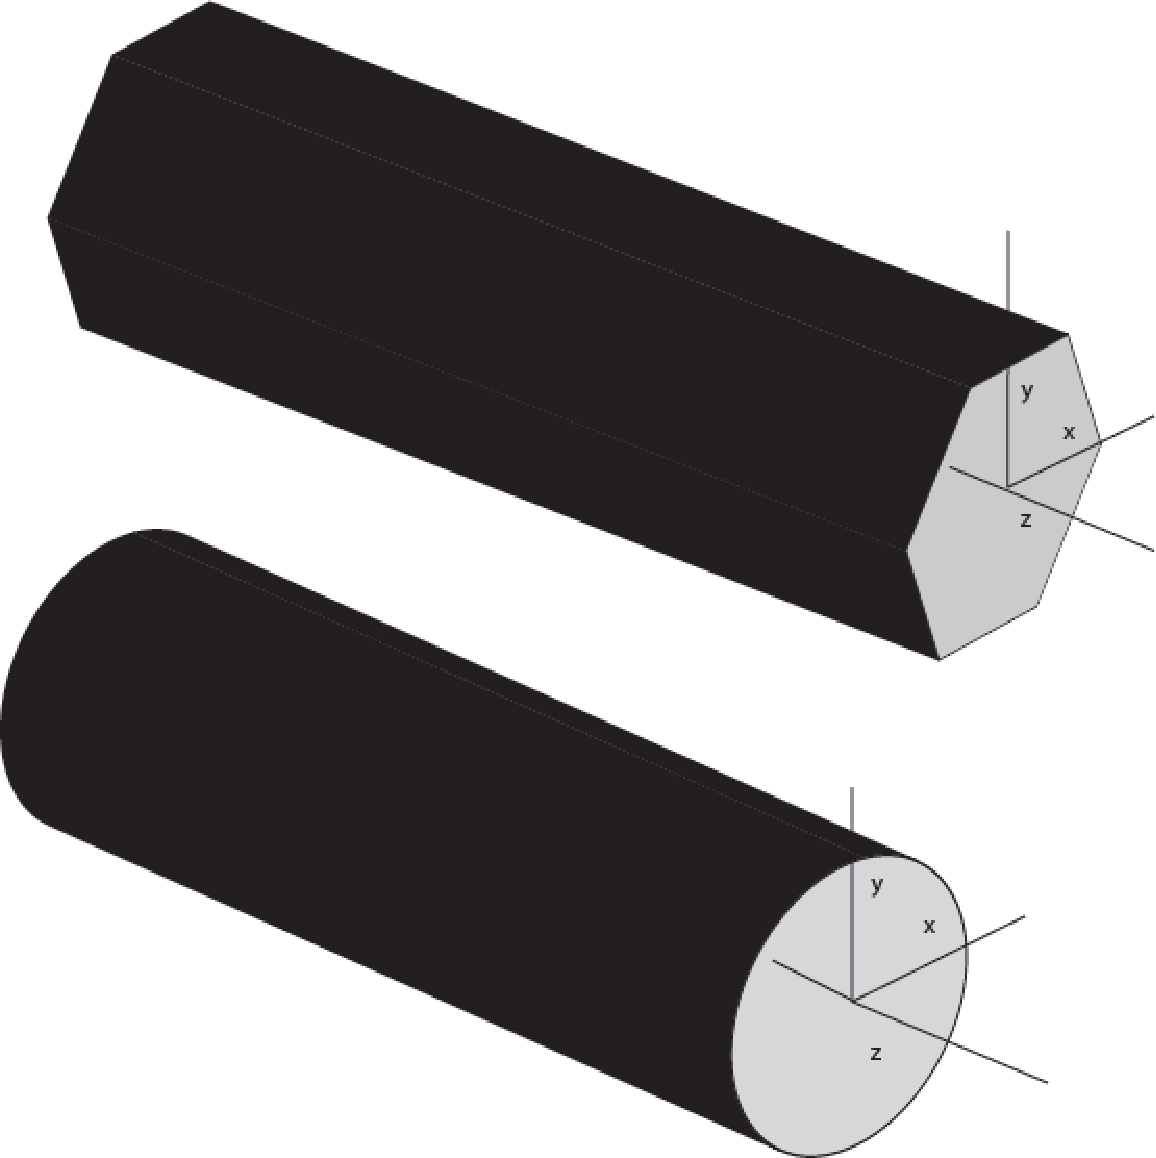
\includegraphics[width=\textwidth]{pictures/LM/NW}
  \label{NW}
\end{figure}

\begin{figure}
  \caption{Geometric Dependence TM radius variation for different Radius and Diameters}
  \centering
  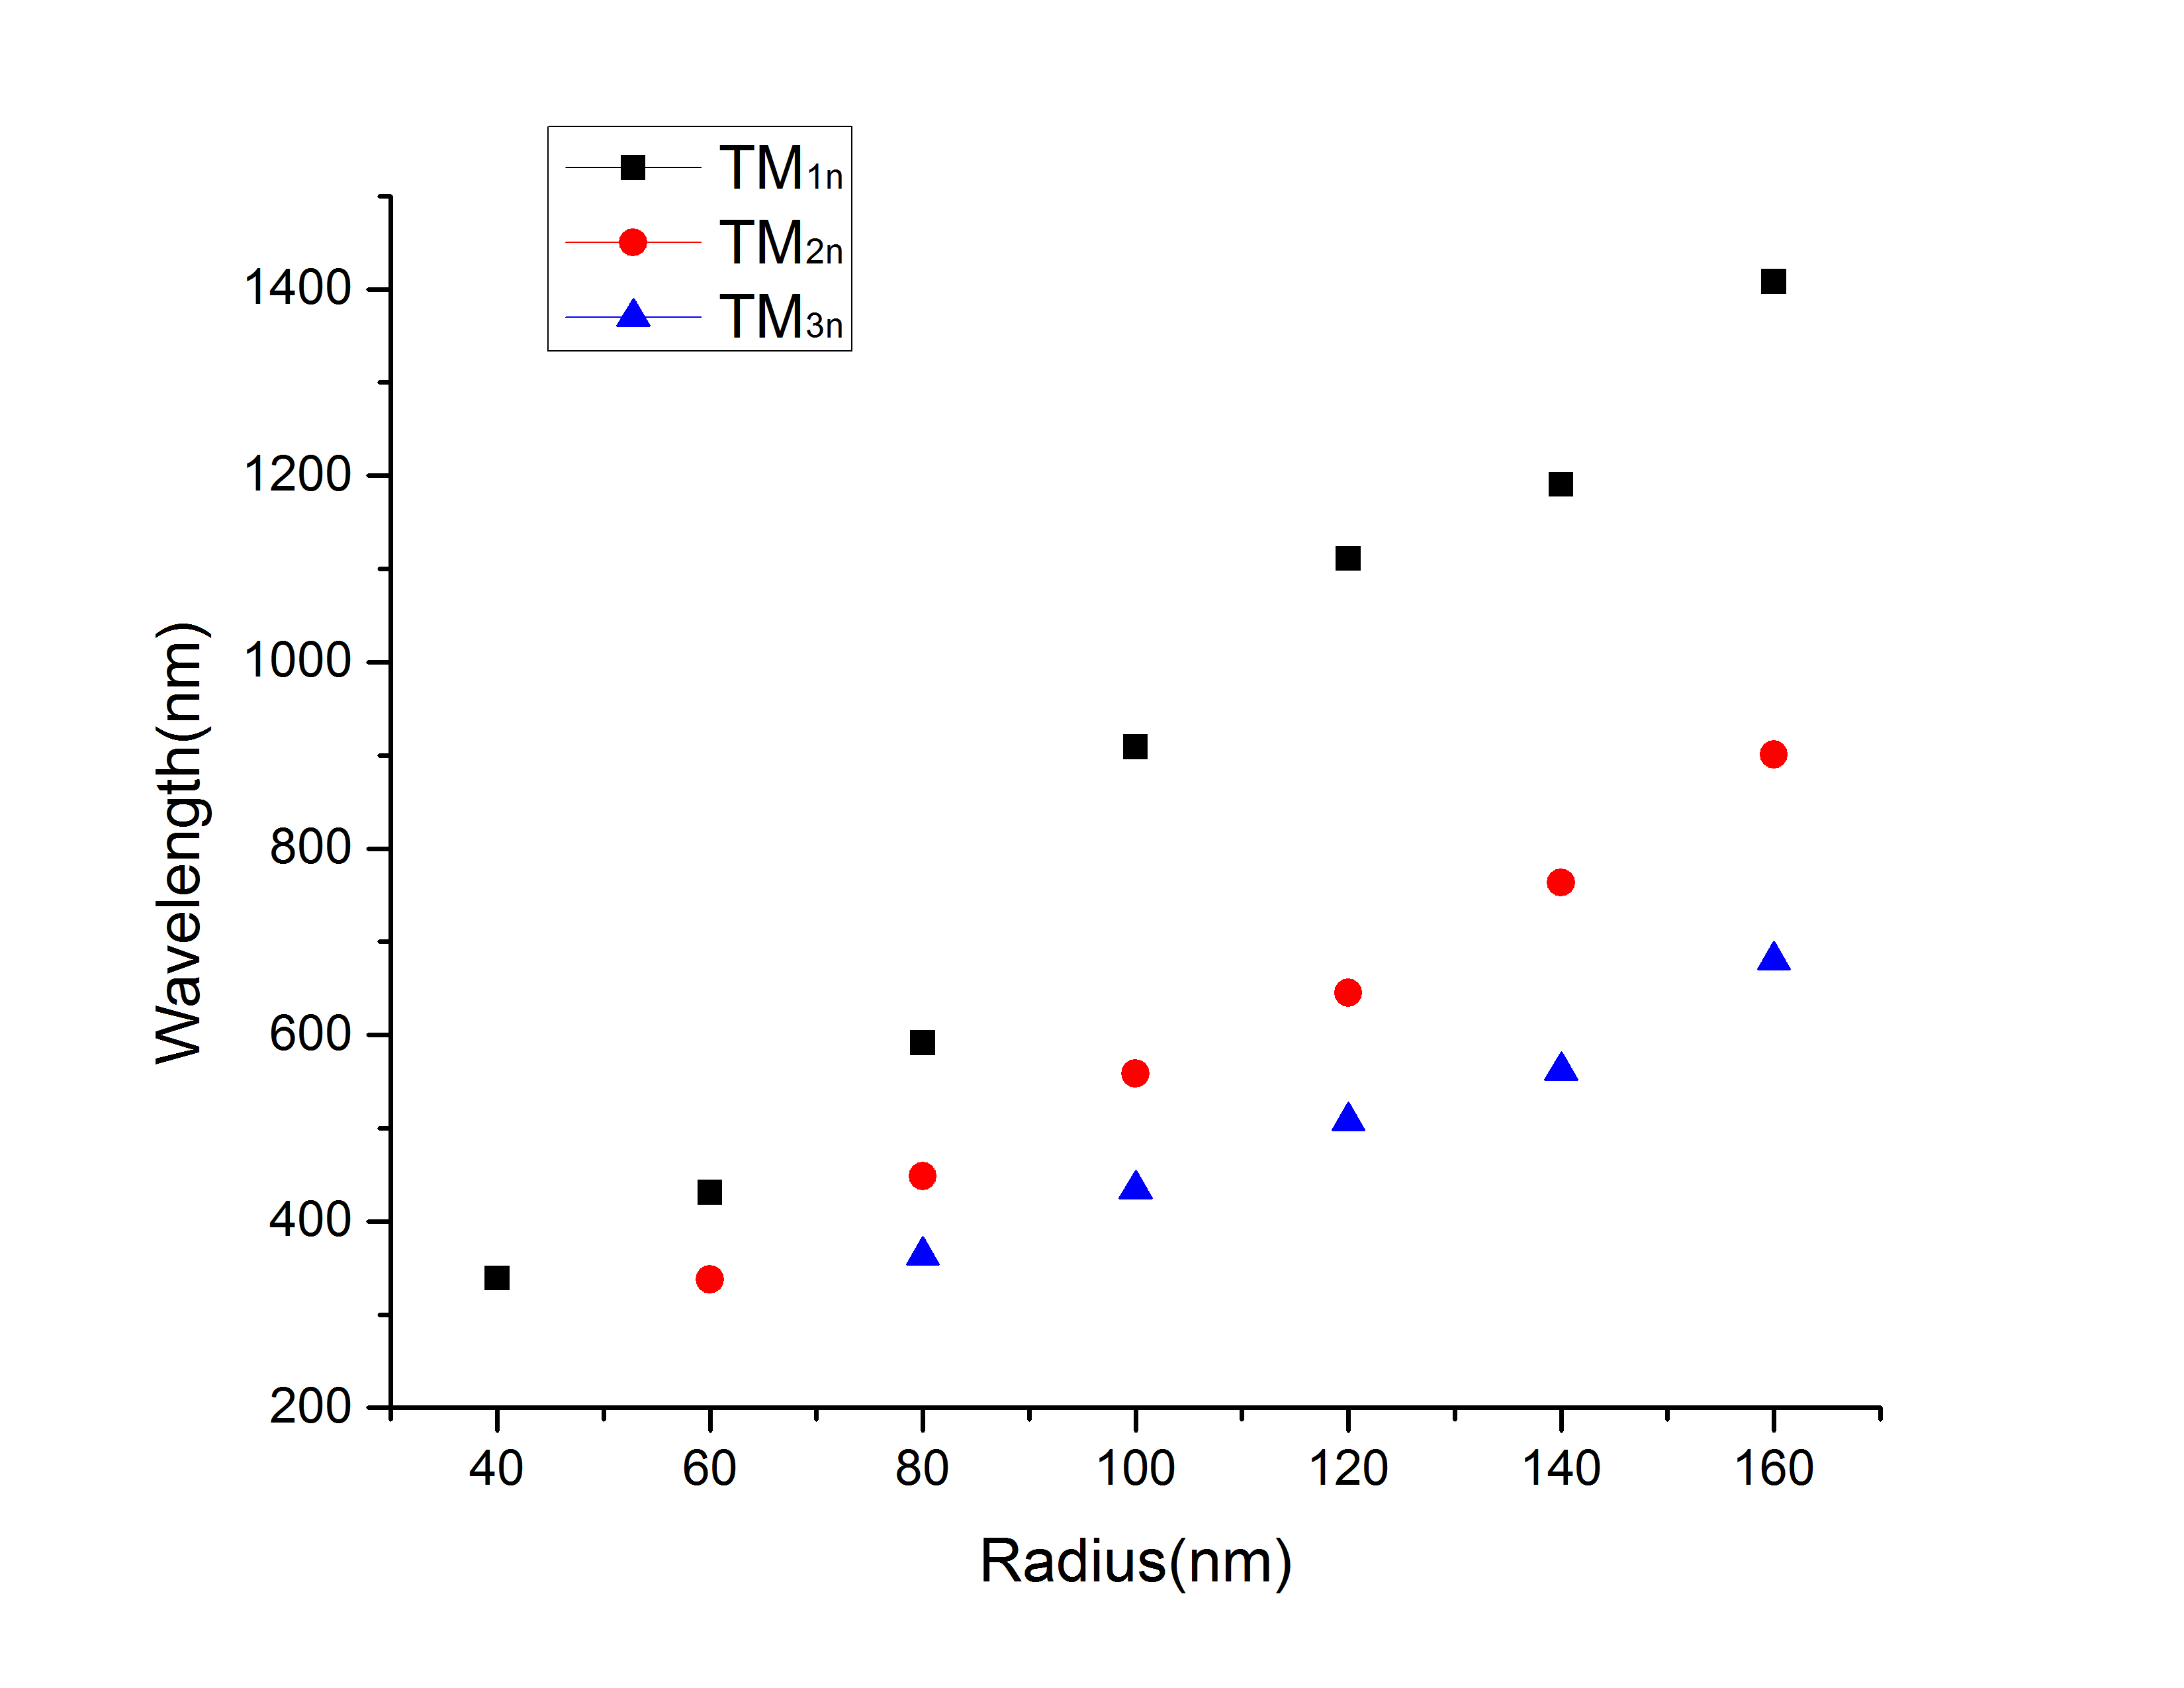
\includegraphics[width=\textwidth]{pictures/LM/TMradius}
  \label{TMradius}
\end{figure}

\begin{figure}
  \caption{Geometric Dependence and Engineering Light with Radius}
  \centering
  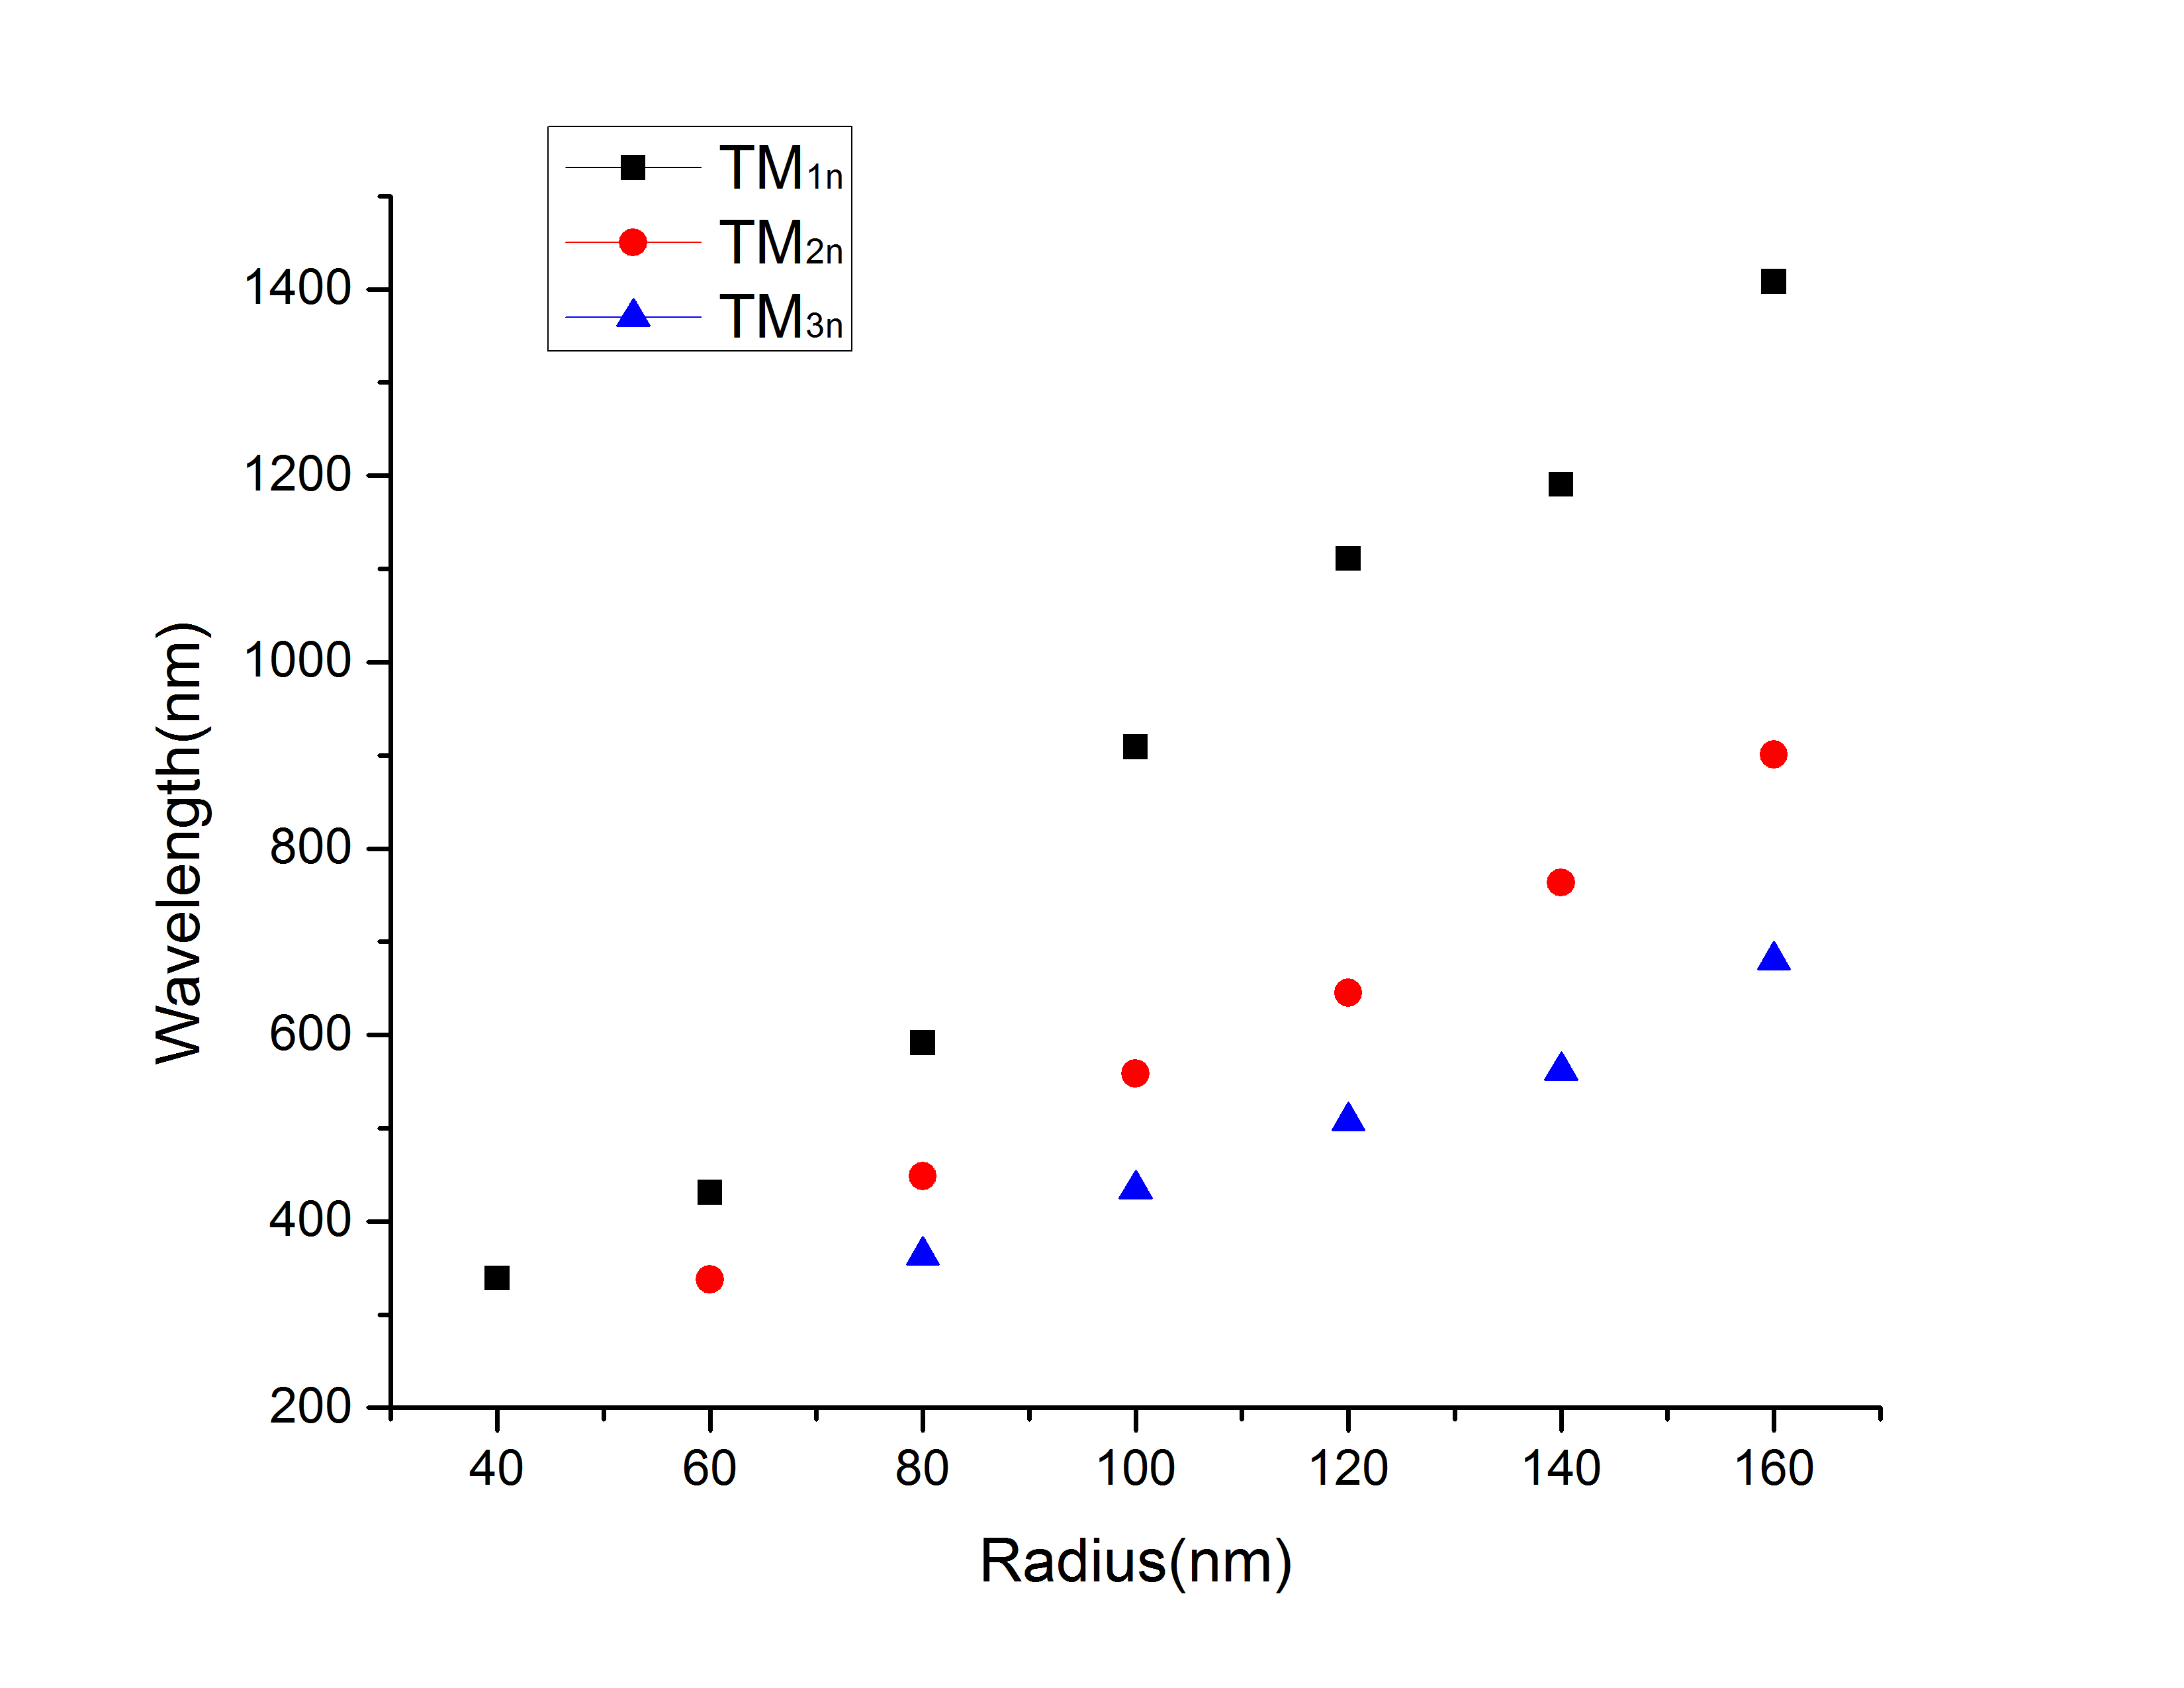
\includegraphics[width=\textwidth]{pictures/LM/TMRadiusScat}
  \label{TMRadiusScat}
\end{figure}

\begin{figure}
  \caption{3D view of Photon Distribution}
  \centering
  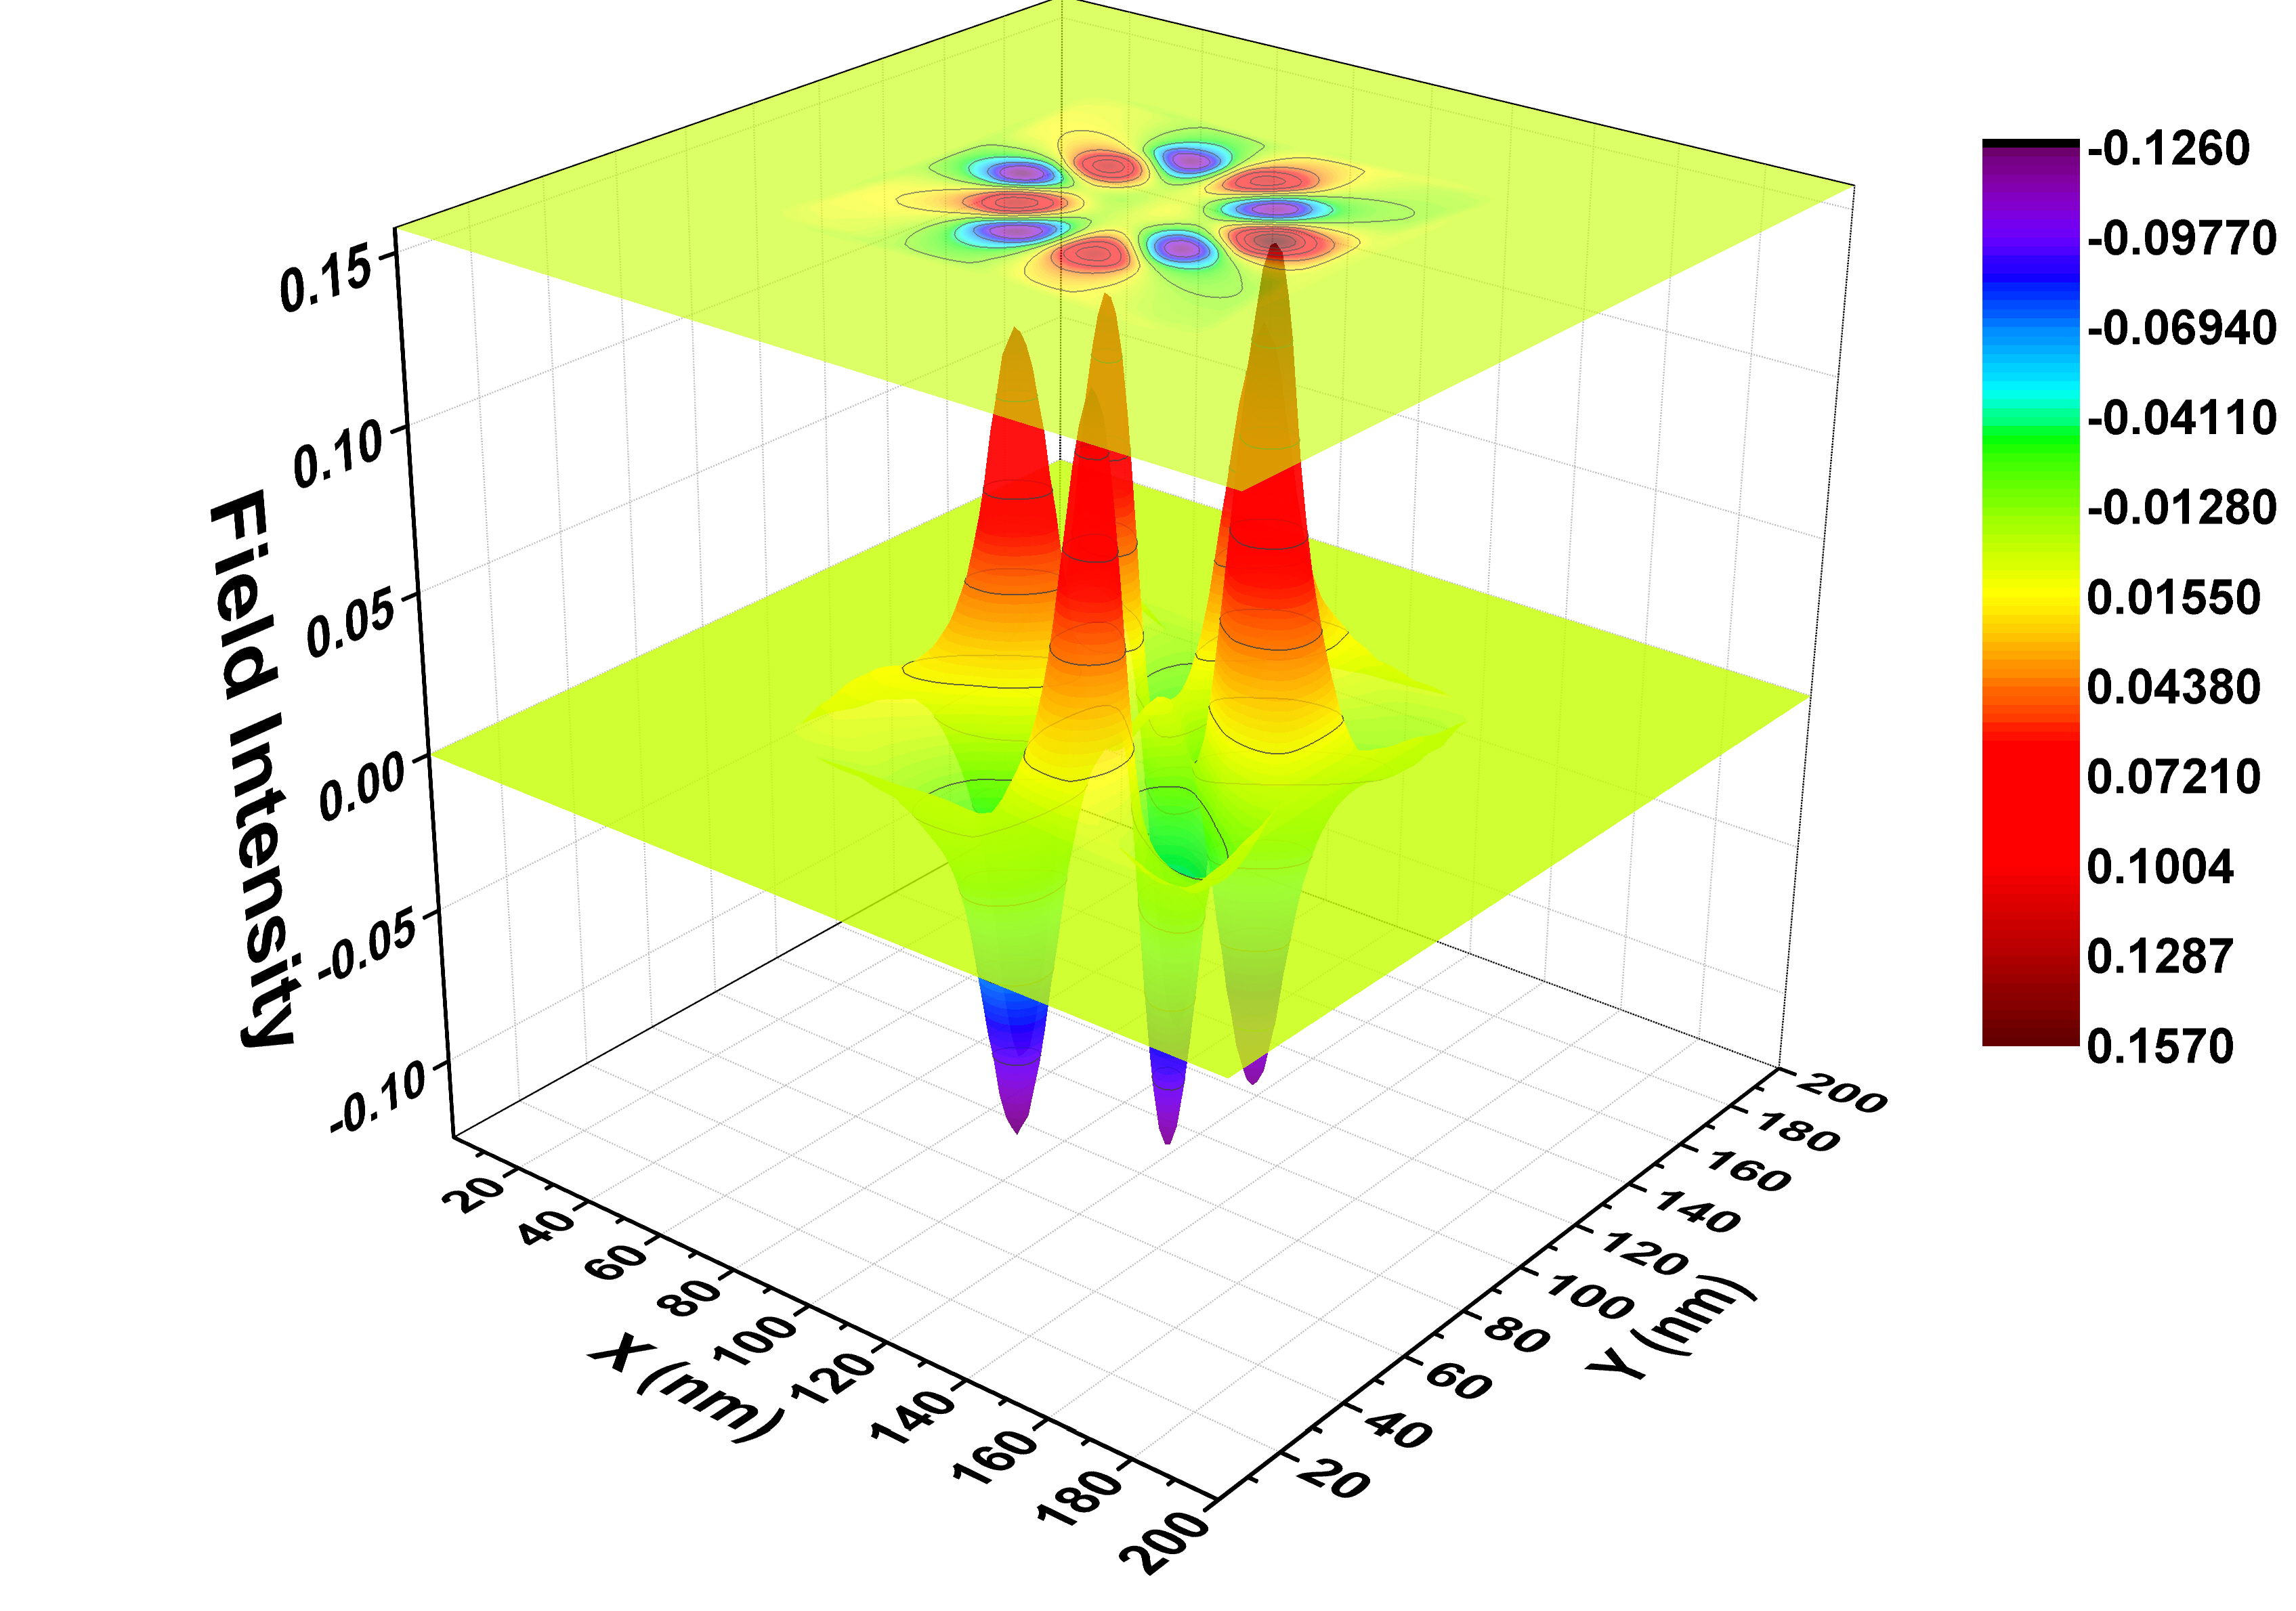
\includegraphics[width=\textwidth]{pictures/LM/photondensity2}
  \label{photondensity2}
\end{figure}
%\subsubsection{\civ-dependent Mean} \label{CIV SED}



